%!TeX root = ../main.tex
\section{Simulación en SciLab}

Partiendo del análisis anterior, se realizará una simulación en SciLab
que permita corroborar los análisis realizados y recuperar los valores
previamente calculados.

El comportamiento del sistema simulado se puede observar en
la gráfica de estados \ref{fig:estados}, la gráfica de salida
\ref{fig:salida} y la gráfica bode \ref{fig:bode}.

\subsubsection{Parámetros del motor}
\begin{lstlisting}[language=Scilab]
R  = 2.1;
L  = 0.005;
Kt = 0.12;
Ke = 0.12;
J  = 0.0001;
B  = 1e-5;
\end{lstlisting}

\subsubsection{Matrices del espacio de estados}
\begin{lstlisting}[language=Scilab]
A = [-R/L,   0, -Ke/L;
        0,   0,     1;
     Kt/J,   0, -B/J];
B = [1/L; 0; 0];
C = [0, 0, 1];
D = 0;
\end{lstlisting}

\subsubsection{Configuración de simulación}
\begin{lstlisting}[language=Scilab]
t0 = 0;
tf = 0.5;
dt = 0.001;
t  = t0:dt:tf;
nt = length(t);
sisMotor = syslin('c', A, B, C, D);
\end{lstlisting}

\subsubsection{Función de transferencia}
\begin{lstlisting}[language=Scilab]
G = ss2tf(sisMotor);
disp("FUNCIÓN DE TRANSFERENCIA G(s):");
disp(G);
\end{lstlisting}

\begin{lstlisting}[style=outputstyle]
FUNCIÓN DE TRANSFERENCIA G(s):
        240000        
   ------------------  
   28842 +420.1s +s^2  
\end{lstlisting}

Resultados en correspondencia con \eqref{eq:TransferFunctionNumeric}

\subsubsection{Simulación de respuesta al escalón}
\begin{lstlisting}[language=Scilab]
u = ones(1, nt);
[y, x] = csim(u, t, sisMotor);
\end{lstlisting}

\subsubsection{Cálculo de autovalores}
\begin{lstlisting}[language=Scilab]
lambda = spec(A);
disp("AUTOVALORES de la matriz A:");
disp("λ₁ = " + string(lambda(1)));
disp("λ₂ = " + string(lambda(2)));
disp("λ₃ = " + string(lambda(3)));
\end{lstlisting}

\begin{lstlisting}[style=outputstyle]
AUTOVALORES de la matriz A:
λ₁ = 0
λ₂ = -333.65826
λ₃ = -86.441738
\end{lstlisting}

En correspondencia con \eqref{eq:ResultadoAutovaloresExperimental}

\subsubsection{Controlabilidad}
\begin{lstlisting}[language=Scilab]
Co = cont_mat(A, B);
rCo = rank(Co);
disp("MATRIZ DE CONTROLABILIDAD (Co):");
disp(Co);
disp("Rango de Co: " + string(rCo));
\end{lstlisting}

\begin{lstlisting}[style=outputstyle]
MATRIZ DE CONTROLABILIDAD (Co):
   200.  -84000.   29520000.
   0.     0.       240000.
   0.     240000.  -1.008D+08
Rango de Co: 3
\end{lstlisting}

En correspondencia con \eqref{eq:MatrizControlabilidadMotorValoresExperimentales}

\subsubsection{Observabilidad}
\begin{lstlisting}[language=Scilab]
Ob = obsv_mat(A, C);
rOb = rank(Ob);
disp("MATRIZ DE OBSERVABILIDAD (Ob):");
disp(Ob);
disp("Rango de Ob: " + string(rOb));
\end{lstlisting}

\begin{lstlisting}[style=outputstyle]
MATRIZ DE OBSERVABILIDAD (Ob):
   0.        0.   1.      
   1200.     0.  -0.1     
  -504120.   0.  -28799.99
Rango de Ob: 2
\end{lstlisting}

En correspondencia con \eqref{eq:MatrizObservabilidadMotorValoresExperimentales}

% ============================================================
% GRÁFICAS CON figure* PARA ANCHO COMPLETO
% ============================================================

\begin{figure*}[tp]
    \centering
    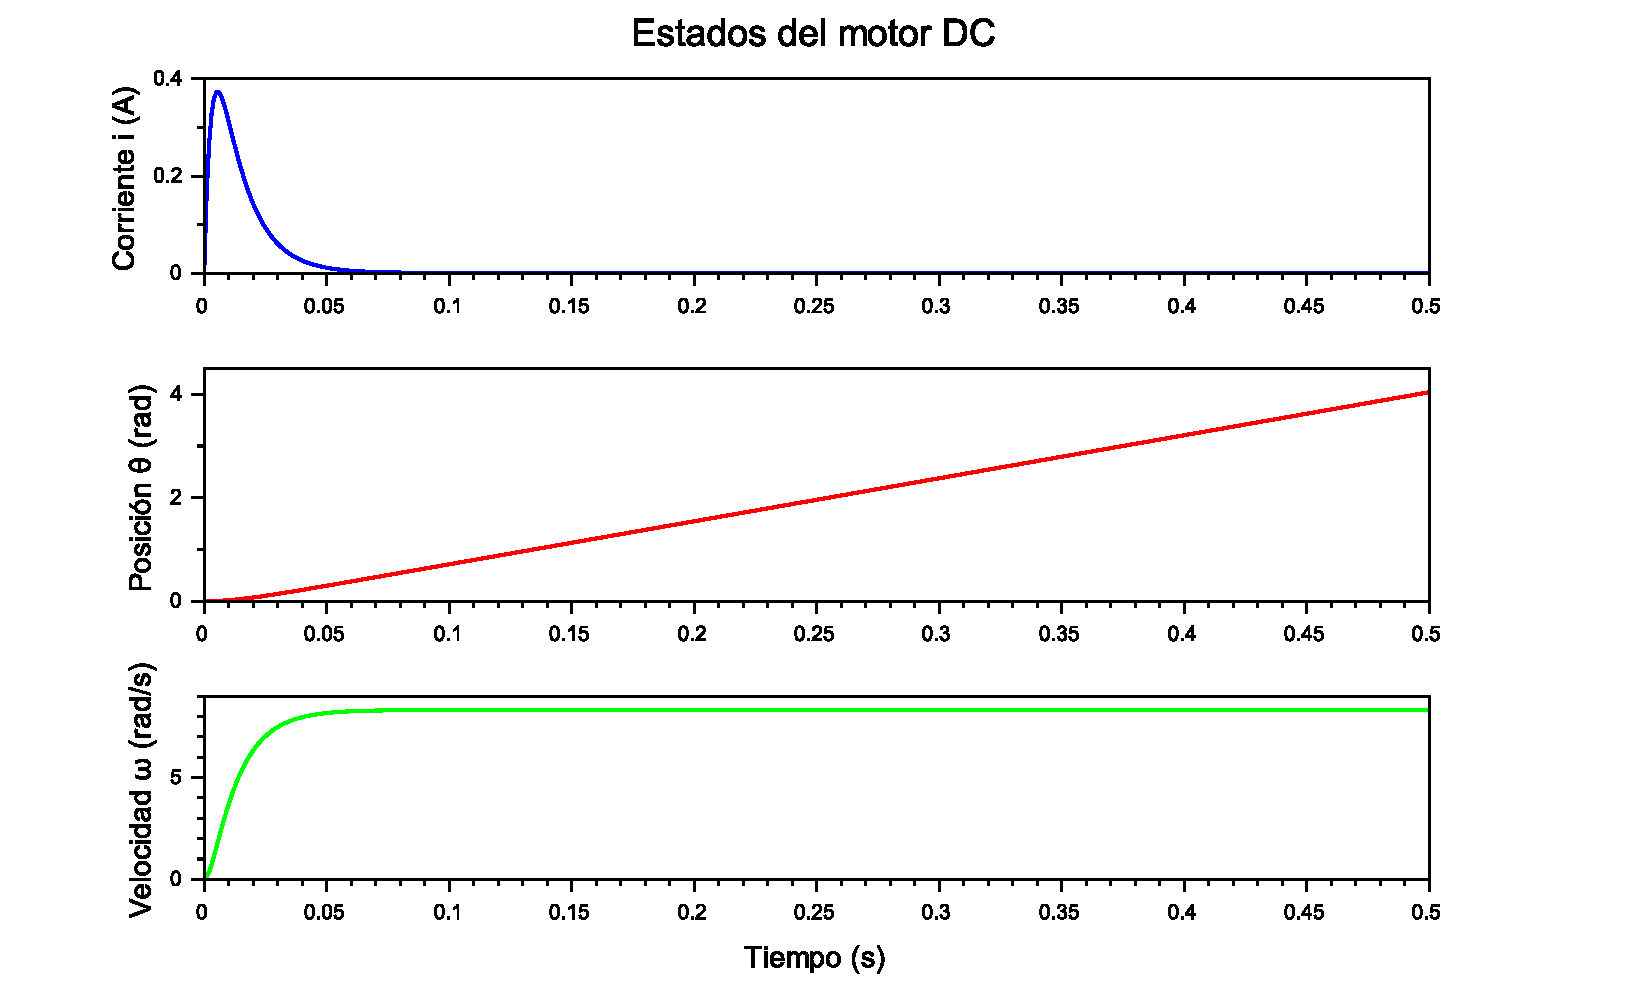
\includegraphics[width=0.95\linewidth]{./img.scilab.eps/estados}
    \caption{Estados del motor DC en respuesta al escalón unitario. Corriente del inducido (azul), posición angular (rojo) y velocidad angular (verde).}
    \label{fig:estados}
\end{figure*}

\begin{figure*}[tp]
    \centering
    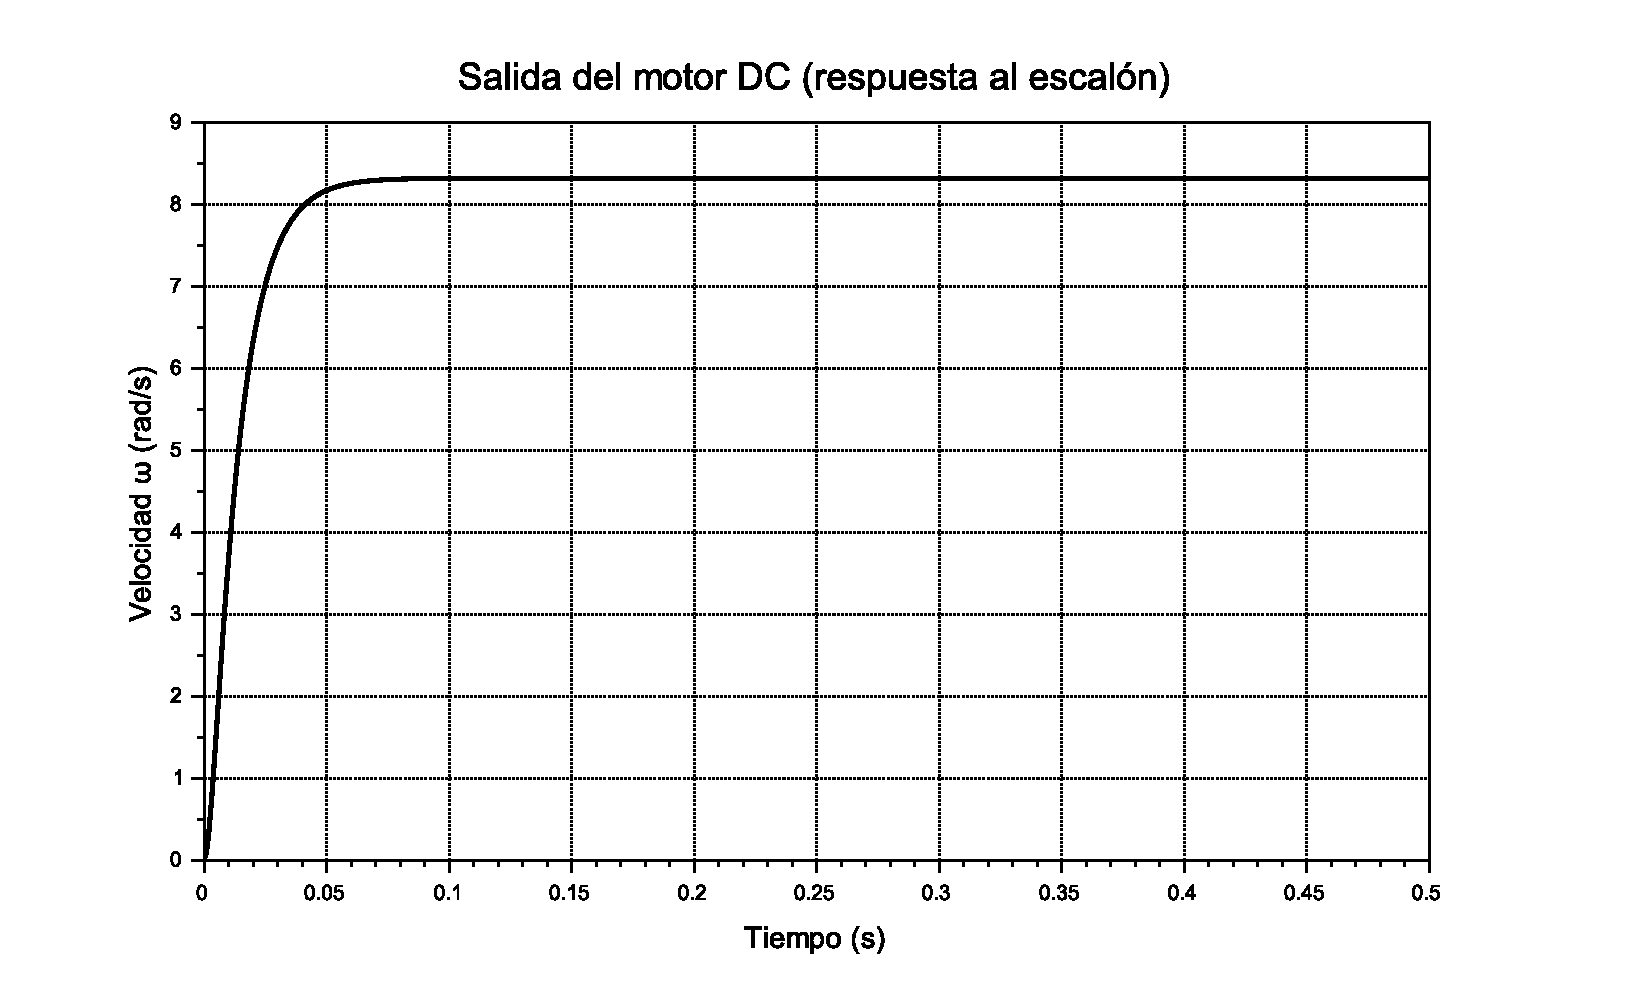
\includegraphics[width=0.95\linewidth]{img.scilab.eps/salida}
    \caption{Salida del sistema: velocidad angular $\omega_m$ en respuesta al escalón de voltaje de entrada $V_{in} = 1$ V.}
    \label{fig:salida}
\end{figure*}

\begin{figure*}[tp]
    \centering
    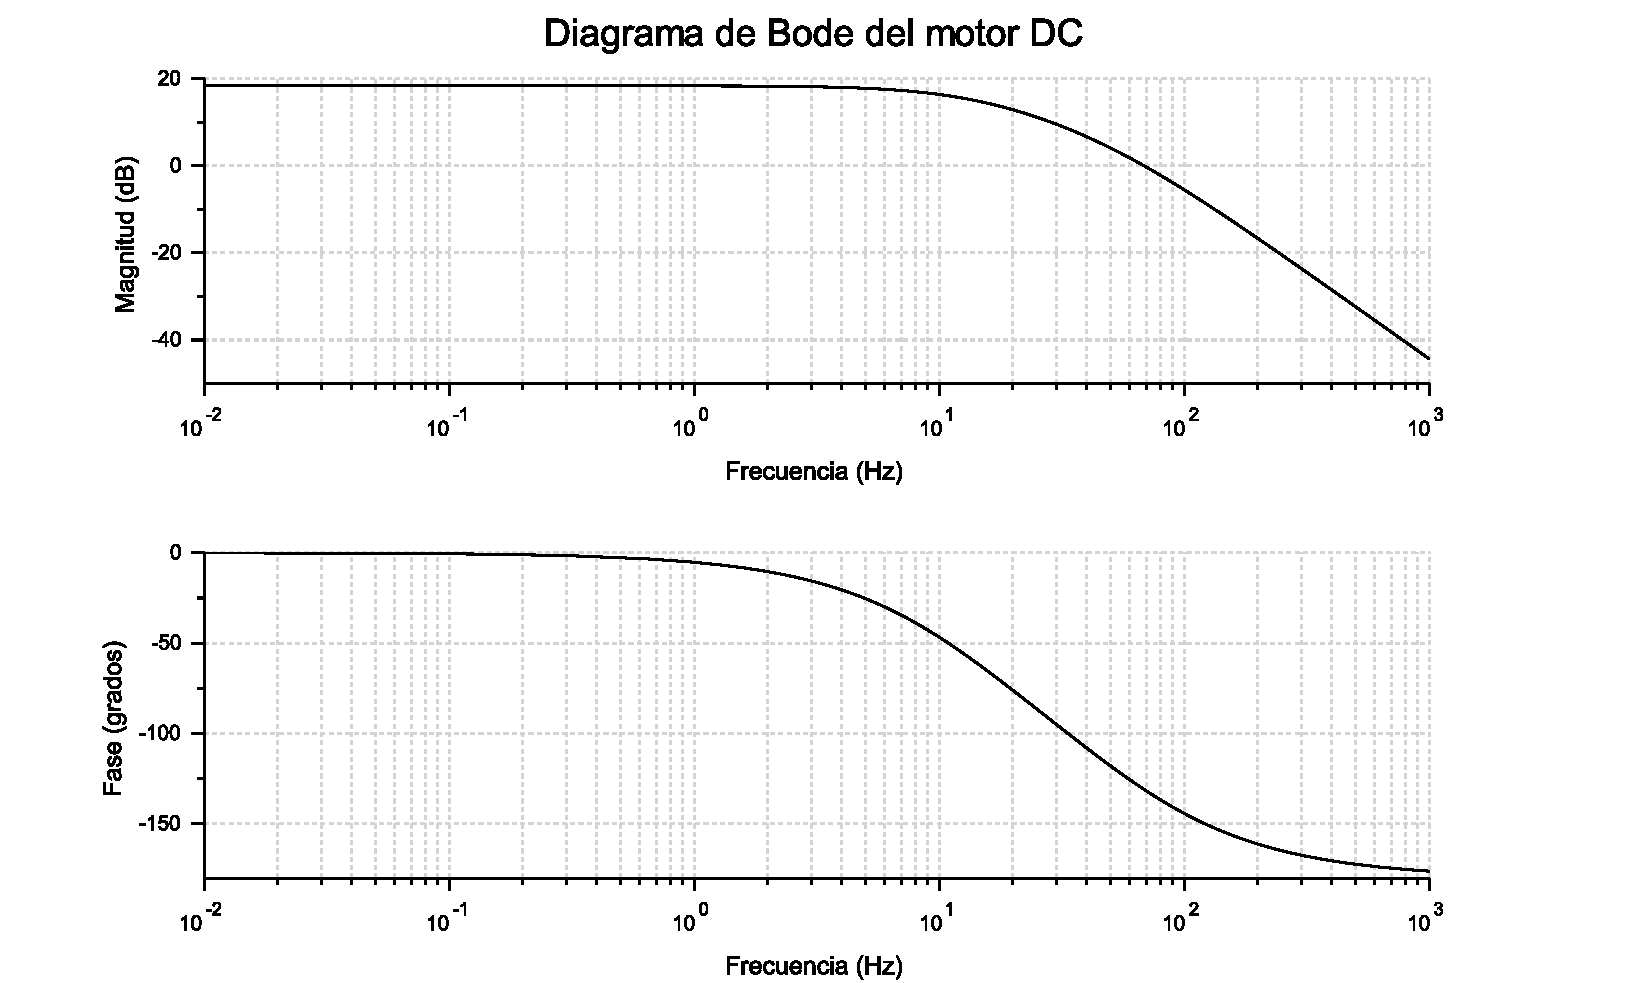
\includegraphics[width=0.95\linewidth]{img.scilab.eps/DiagramaBodeMotorDC}
    \caption{Diagrama de Bode del sistema motor DC. Magnitud (superior) y fase (inferior) en función de la frecuencia.}
    \label{fig:bode}
\end{figure*}

%\begin{figure*}[t]
%    \centering
%    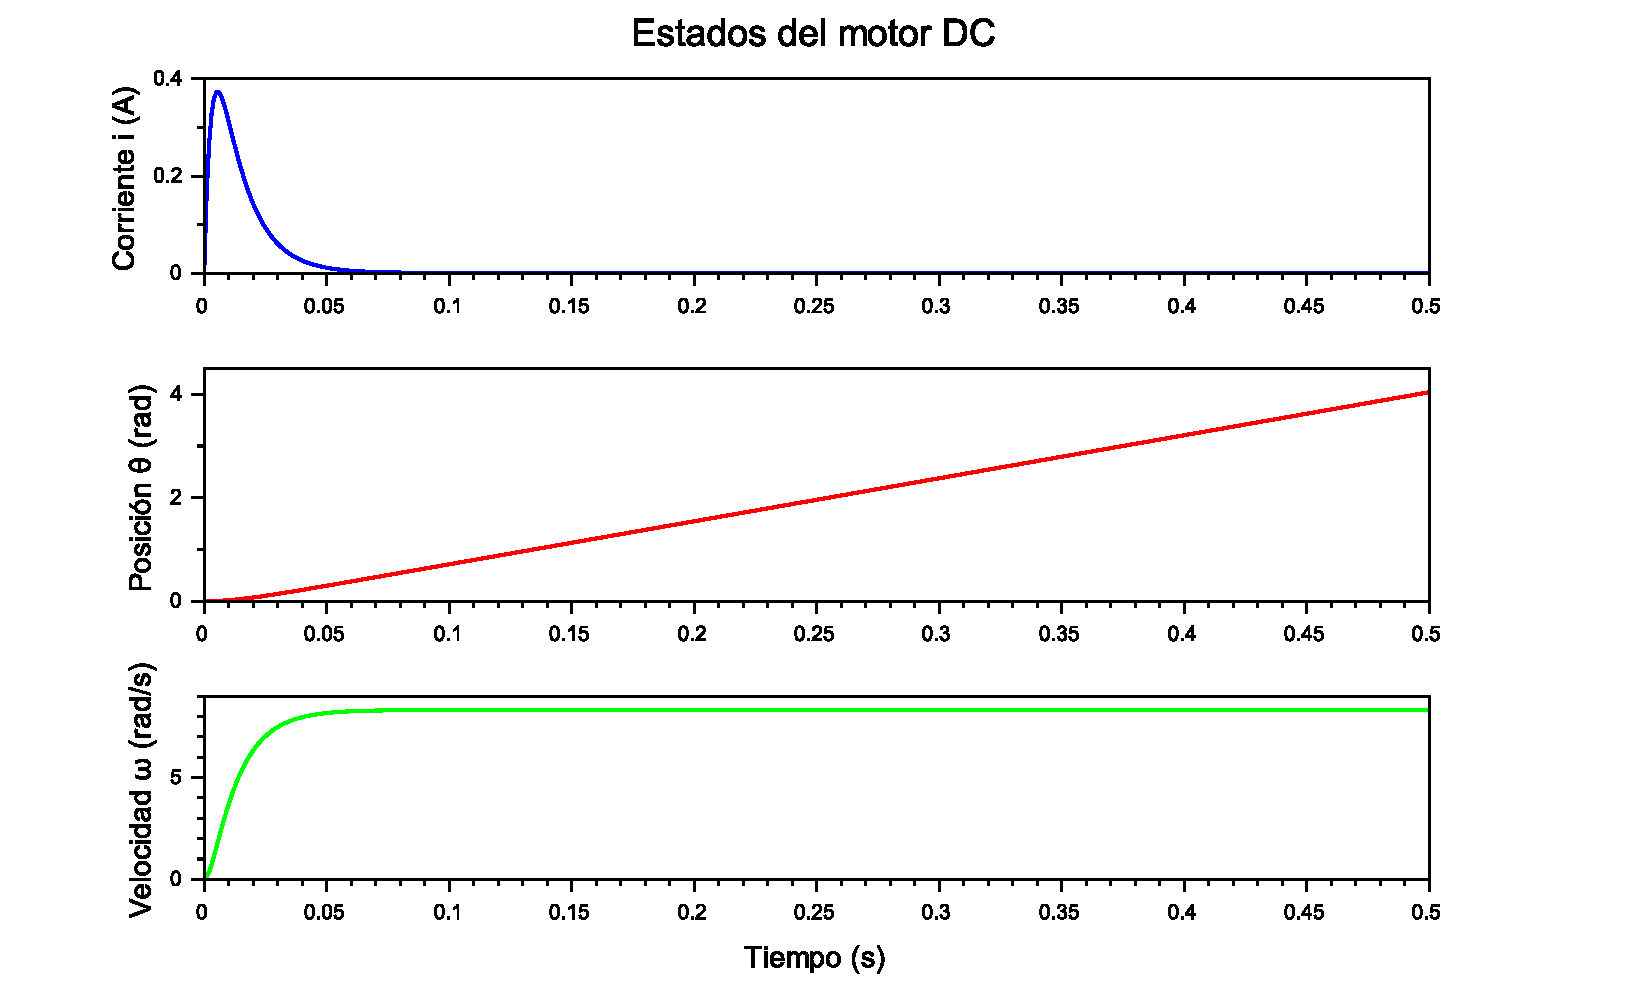
\includegraphics[width=0.95\linewidth]{./img.scilab.eps/estados}
%    \caption{Estados del motor DC en respuesta al escalón unitario. Corriente del inducido (azul), posición angular (rojo) y velocidad angular (verde).}
%    \label{fig:estados}
%\end{figure*}
%
%\begin{figure*}[t]
%    \centering
%    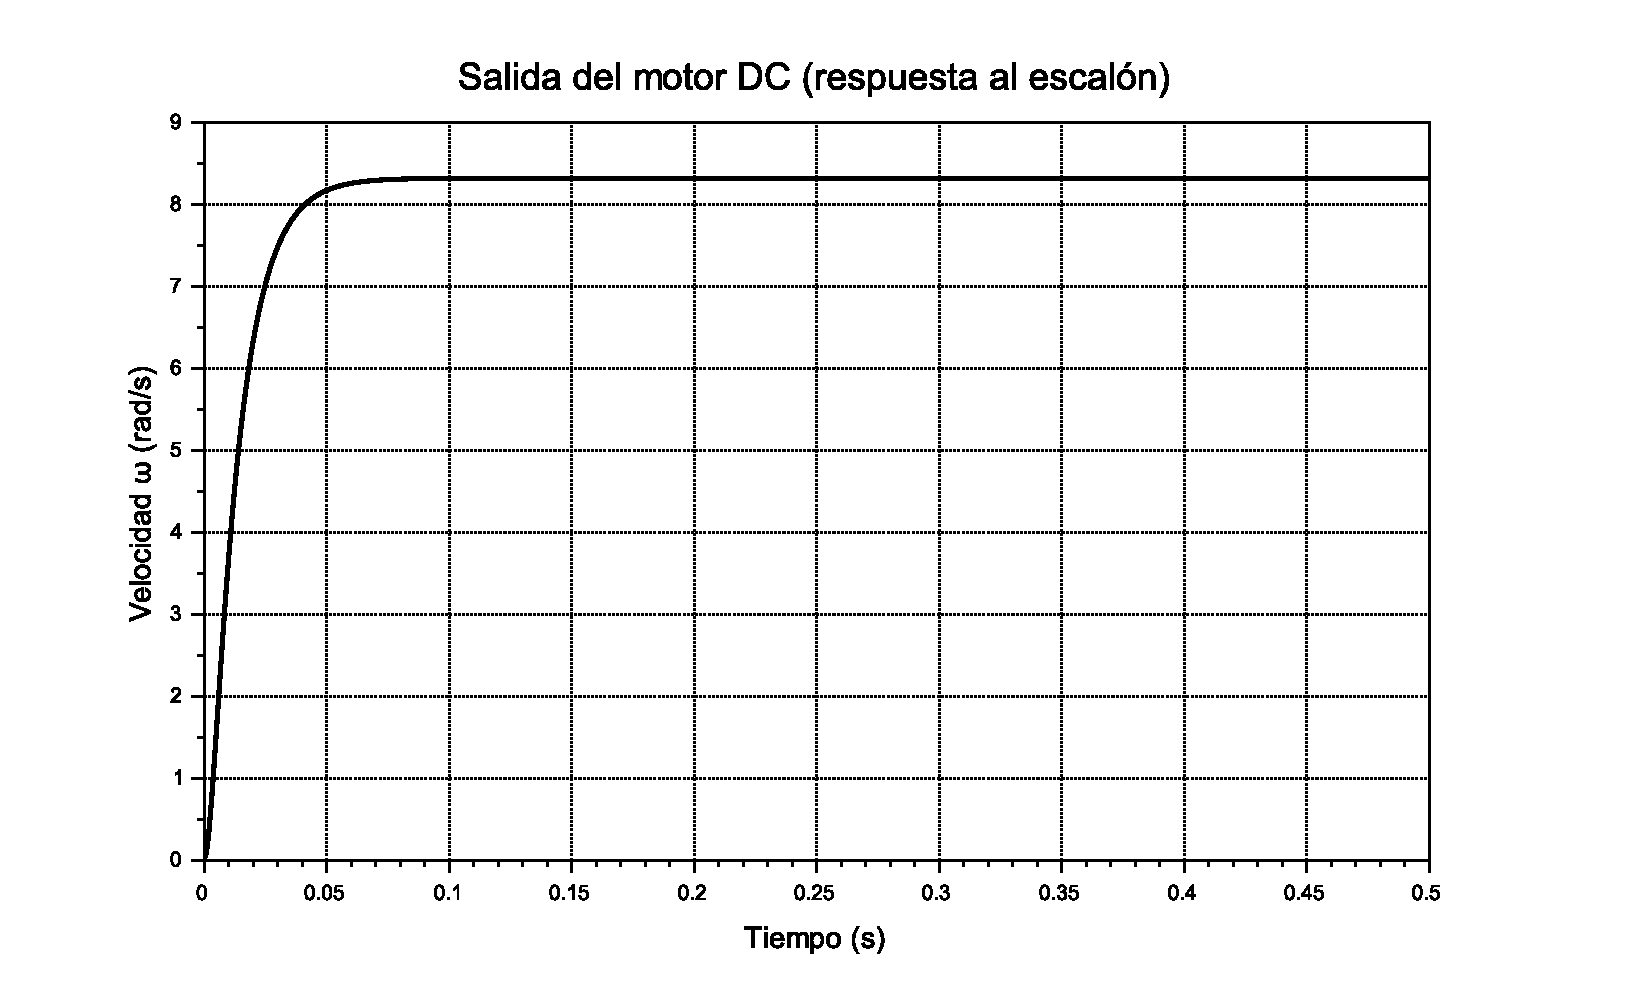
\includegraphics[width=0.95\linewidth]{img.scilab.eps/salida}
%    \caption{Salida del sistema: velocidad angular $\omega_m$ en respuesta al escalón de voltaje de entrada $V_{in} = 1$ V.}
%    \label{fig:salida}
%\end{figure*}
%
%\begin{figure*}[t]
%    \centering
%    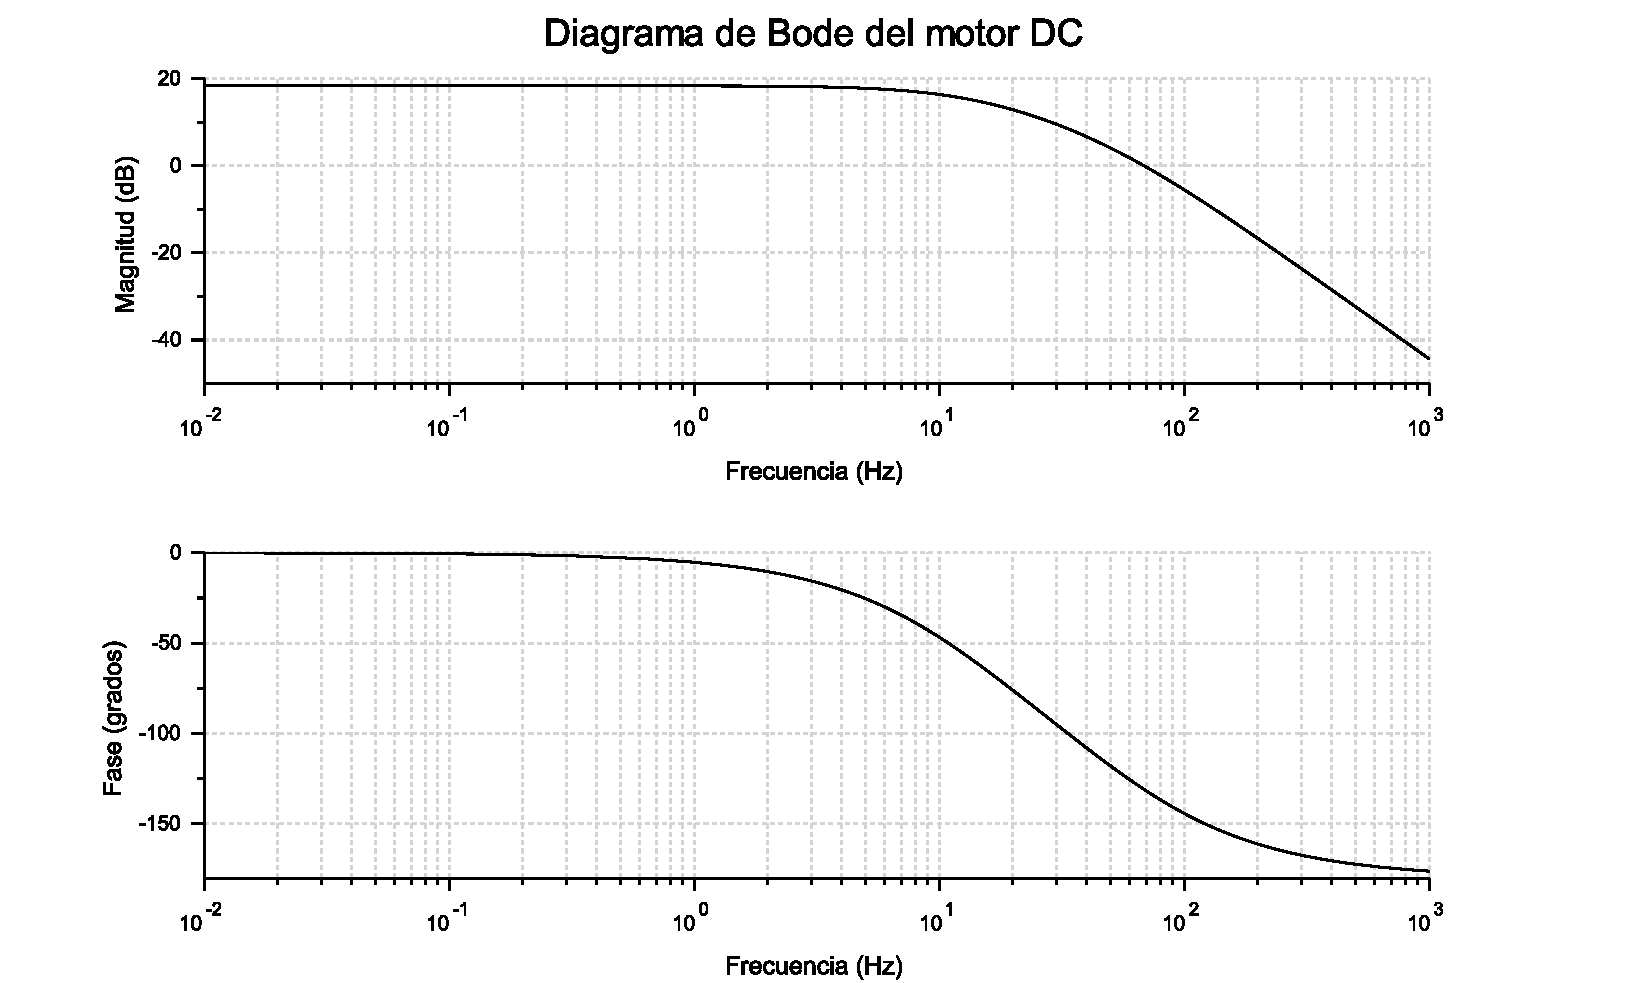
\includegraphics[width=0.95\linewidth]{img.scilab.eps/DiagramaBodeMotorDC}
%    \caption{Diagrama de Bode del sistema motor DC. Magnitud (superior) y fase (inferior) en función de la frecuencia.}
%    \label{fig:bode}
%\end{figure*}
